
% This LaTeX was auto-generated from MATLAB code.
% To make changes, update the MATLAB code and republish this document.

\documentclass[11pt]{article}
\usepackage[utf8]{inputenc}
\usepackage[T1]{fontenc}
\usepackage{amsthm}
\usepackage{enumitem}
\usepackage{amssymb}
\usepackage{amsmath}
\usepackage{amsfonts}
\usepackage[version=4]{mhchem}
\usepackage{stmaryrd}
\usepackage{mathrsfs}
\usepackage{bm}
\usepackage{graphicx}
\usepackage[export]{adjustbox}
\graphicspath{ {./images/} }
\usepackage{algorithm}
\usepackage{algorithmic}
\usepackage{makecell}  % 表格换行
\usepackage{tikz}

\usepackage{hyperref}
\hypersetup{
    colorlinks=true,     % 启用颜色链接
    linkcolor=black,     % 内部链接的颜色
    citecolor=blue,      % 引用文献的颜色
    urlcolor=blue,       % URL链接的颜色
    linktoc=red,      % 不影响目录链接颜色
}

\usepackage[a4paper, top=1in, bottom=1in, left=1in, right=1in]{geometry}

\title{
{\bf \huge Exercises Review}
%{\bf \large For M\"untz systems on [0,1]}
}
\author{Huaijin Wang}
\date{May 28, 2025}





\begin{document}


\newtheorem{definition}{Definition}[section]
\newtheorem{property}{Property}[section]
\newtheorem{lemma}{Lemma}[section]
\newtheorem{theorem}{Theorem}[section]
\newtheorem{corollary}{Corollary}[section]
\newtheorem{remark}{Remark}[section]
\newtheorem{example}{Example}[]
\newtheorem{notation}{Notation Declaration}[]
\newtheorem{question}{Question}[]
\newtheorem{exercise}{Exercise}[section]
\newtheorem{exercise*}{Exercise}[]

\maketitle

\tableofcontents


\newpage


\setcounter{section}{0}
\section{Week 4}

\setcounter{section}{2}
\setcounter{exercise}{13}
\begin{exercise}
Consider the elliptic problem
\[
\left\{
\begin{aligned}
& L  u  : =  -u_{xx} + u_x + u =f, \quad \forall x\in (a,b),\\
& u(a) = u(b) = 0,
\end{aligned}
\right .
\]
and its finite difference schema 
\begin{equation}
\left \{
\begin{aligned}
L_h u_i :=   -\frac{u_{i+1} - 2u_i + u_{i-1}}{h^2} + \frac{u_{i+1} - u_{i-1}}{2h} + u_i = f_i, & \quad \forall i=1,\cdots,N-1, \\
 u_0 = u_N = 0, & \\ 
 \end{aligned}
\right .
 \label{eq:2-14}
\end{equation}
in an uniform mesh $\{x_i \}_{i=0}^N$, $x_i = a+ih$, $h = (b-a)/N$. \\
$1).$ Derive an estimate for the truncation error; \\
$2).$ Establish an a priori estimate for $\|u_h\|_1$; \\
$3).$ Prove the existence and uniqueness of the solution of the finite difference schema; \\
$4).$ Derive an  error estimate for $\|e_h\|_1$, where $e_i = u(x_i) - u_i$.
\end{exercise}
\begin{proof}[Solution]
1). The truncation error is 
\[
R_i = L_h [u(x_i)] - [L u] (x_i) = -\left(\frac{u(x_{i+1}) - 2u(x_i) + u(x_{i-1})}{h^2}-u_{xx}(x_i) \right)+ \frac{u(x_{i+1}) - u(x_{i-1})}{2h} - u_x(x_i),
\]
where $ i=1,\cdots,N-1$.
 By the Tylor developments
\[
u(x_{i+1}) = u(x_i) + h u^\prime(x_i) + \frac{h^2}{2} u^{\prime \prime} (x_i) + \frac{h^3}{3!} u^{(3)} (x_i) + \frac{h^4}{4!} u^{(4)} (\xi_i), \ \text{for some} \ \xi_i \in (x_i, x_{i+1}),
\]
\[
u(x_{i-1}) = u(x_i) - h u^\prime(x_i) + \frac{h^2}{2} u^{\prime \prime} (x_i) - \frac{h^3}{3!} u^{(3)} (x_i) + \frac{h^4}{4!} u^{(4)} (\eta_i), \ \text{for some} \ \eta_i \in (x_{i-1},x_{i}),
\]
we obtain that $R_i = O(h^2)$ as $h \to 0$ for $i=1,\cdots,N-1$. 

 \vspace{1em}

2). We introduce some results in discrete form first (see [slides part1.pdf, pp. 41-48]).
\textcolor{gray}{
\begin{enumerate}[label=(\roman*)]
\item Sets of noses:
\[
I_h = \{x_1,\cdots,x_{N-1}\}, \ \bar{I}_h = \{x_0,x_1,\cdots, x_N\}, \ I_h^+ = \{x_1,\cdots,x_N\}.
\]
\item Grid spacing: $h = h_i := x_{i}- x_{i-1}, \ i=1,\cdots,N$, and
\[
\begin{aligned}
&\bar{h}_0  = \frac{1}{2} h_1, \ \bar{h}_N = \frac{1}{2} h_N,\quad \bar{h}_i = \frac{1}{2} (h_i+h_{i+1}), \ i=1,\cdots,N-1.
\end{aligned}
\]
\item Discrete functions: $v_h = \{v_0,v_1,\cdots, v_N \}$ defined on $\bar{I}_h$.
\item Difference operators: 
\[
\begin{aligned}
& (v_i)_{\bar{x}} := v_{i,\bar{x}} : = \frac{v_i-v_{i-1}}{h_i}, \ i =1,\cdots,N, \\
& (v_i)_x := v_{i, x} := \frac{v_{i+1} - v_i}{h_{i+1}},\ i=0,\cdots,N-1, \\
&  (v_i)_{\hat{x}} := v_{i, \hat{x}} := \frac{v_{i+1} - v_i}{\bar{h}_{i}},\ i=0,\cdots,N-1.
\end{aligned}
\]
\item Discrete inner products:
\begin{equation}
(u_h, v_h)_{I_h} = \sum_{i=1}^{N-1} u_i v_i \bar{h}_i, \
(u_h, v_h)_{\bar{I}_h} = \sum_{i=0}^{N} u_i v_i \bar{h}_i, \
(u_h, v_h)_{I^+_h} = \sum_{i=1}^{N} u_i v_i h_i.
\label{eq:d-ip}
\end{equation}
\item Discrete norms:
\begin{equation}
\begin{aligned}
& \|v_h\|_c := \max_{\bar{I}_h} |v_i|,\ \|v_h\|_0 := (v_h,v_h)_{\bar{I}_h}^{1/2}, \\
& |v_h|_1 := ((v_h)_{\bar{x}}, (v_h)_{\bar{x}})_{I_h^+}^{1/2}, \ \|v_h\|_1^2 = \|v_h\|_0^2 + |v_h|_1^2.
\end{aligned}
\label{eq:d-in}
\end{equation}
\end{enumerate}
We have some conclusions:
\begin{enumerate}[label=(\roman*)]
\item Discrete integral by parts (see [slides part1.pdf, p. 44]).
\begin{equation}
\sum_{i=m+1}^n v_i (w_i)_{\bar{x}} h_i = - \sum_{i=m}^{n-1} (v_i)_x w_i h_{i+1} + v_n w_n - v_m w_m,\quad 0\leqslant m < n \leqslant N.
\label{eq:d-ibp}
\end{equation}
\item Discrete Green formula (see [slides part1.pdf, p. 45]).
\begin{equation}
\sum_{i=m+1}^{n-1} \left( (u_i)_{\bar{x}} \right )_{\hat{x}} v_i \bar{h}_i = - \sum_{i=m+1}^n (u_i)_{\bar{x}} (v_i)_{\bar{x}} h_i + (u_n)_{\bar{x}} v_n - (u_m)_x v_m, \quad  0\leqslant m < n \leqslant N.
\label{eq:d-gf}
\end{equation}
\item Discrete Cauchy-Schwarz inequality (see [slides part1.pdf, p. 47]).
\begin{equation}
|(u_h, v_h)_{\bar{I}_h}| \leqslant (u_h, u_h)_{\bar{I}_h}^{1/2} (v_h, v_h)_{\bar{I}_h}^{1/2}.
\label{eq:d-csi}
\end{equation}
\item Discrete Poincar\'e inequalities (see [slides part1.pdf, pp. 47-48] and [HW 3, Exercise 2.12]). 
Assume that $v_0 = 0$ or $v_N=0$,
\begin{equation}
\|v_h\|_c \leqslant C |v_h|_1, \quad \|v_h\|_0 \leqslant C |v_h|_1,
\label{eq:d-pi}
\end{equation}
where $C$ is a constant depending only on $a$ and $b$.
\end{enumerate}
}

Note that 
\[
L_h u_i 
 = -\left(\left(u_i\right)_{\bar{x}}\right)_{\hat{x}}+\frac{1}{2}\left(\left(u_i\right)_{\bar{x}}+\left(u_i\right)_x\right)+u_i,\quad i=1,\cdots,N-1.
\]
Multiplying both sides of the finite difference schema $L_h u_i = f_i$ by $u_i h_i$ yields
\[
-\left(\left(u_i\right)_{\bar{x}}\right)_{\hat{x}} u_i h_i + \frac{1}{2} \left(\left(u_i\right)_{\bar{x}}+\left(u_i\right)_x\right) u_i h + u_i^2 h = f_i u_i h_i,\quad \forall i=1,\cdots,N-1.
\]
Summing in $i$ from $1$ to $N-1$ gives
\[
- \left(\left(\left(u_h\right)_{\bar{x}}\right)_{\hat{x}}, u_h \right )_{I_h} + \frac{1}{2} \left( (u_h)_{\bar{x}} + (u_h)_{x}, u_h \right)_{I_h}  + \left( u_h , u_h \right)_{I_h}= (f_h, u_h)_{I_h}.
\]
In virtue of discrete integral by parts \eqref{eq:d-ibp}, discrete Green formula \eqref{eq:d-gf} and the fact that $u_0 = u_N = 0$, we have 
\[
- \left (\left(\left(u_h\right)_{\bar{x}}\right )_{\hat{x}}, u_h \right)_{I_h}  =  \left( (u_h)_{\bar{x}}, (u_h)_{\bar{x}} \right)_{I_h^+}, \quad \left( (u_h)_{\bar{x}}, u_h \right)_{I_h} = - \left( (u_h)_x, u_h \right)_{I_h} .
\]
\textcolor{gray}{
In fact, set $m=0$ and $n=N$ in discrete Green formula \eqref{eq:d-gf}, we have
\[
- \left (\left(\left(u_h\right)_{\bar{x}}\right )_{\hat{x}}, u_h \right)_{I_h} 
= -\sum_{i=1}^{N-1}  (u_i)_{\bar{x}} )_{\hat{x}} u_i h 
= \sum_{i=1}^{N-1} (u_i)_{\bar{x}} (u_i)_{\bar{x}} h - (u_N)_{\bar{x}} u_N + (u_0)_{\bar{x}} u_0 =  \left( (u_h)_{\bar{x}}, (u_h)_{\bar{x}} \right)_{I_h^+}.
\]
And set $m=0$ and $n=N$ in  discrete integral by parts \eqref{eq:d-ibp}, we have
\[
\begin{aligned}
& \left( (u_h)_{\bar{x}}, u_h \right)_{I_h} = \sum_{i=1}^{N-1} (u_i)_{\bar{x}} u_i h
= \sum_{i=1}^{N} (u_i)_{\bar{x}} u_i h
= -\sum_{i=0}^{N-1} (u_i)_{x} u_i h + (u_N)^2-(u_0)^2 \\
& = -\sum_{i=1}^{N-1} (u_i)_{x} u_i h = - ( (u_h)_{x}, u_h)_{I_h}.
\end{aligned}
\]
}
Thus 
\[
\left( (u_h)_{\bar{x}}, (u_h)_{\bar{x}} \right)_{I_h^+} + \left (u_h,u_h \right )_{I_h} = \left (f_h, u_h \right)_{I_h}.
\]
Using the fact that $u_0=u_N=0$, it is equivalent to
\[
\left( (u_h)_{\bar{x}}, (u_h)_{\bar{x}} \right)_{I_h^+} + \left (u_h,u_h \right )_{\bar{I}_h} = \left (f_h, u_h \right)_{\bar{I}_h}.
\]
By the definition of the discrete inner norm \eqref{eq:d-in}, the left-hand side of the above formula is $\|u_h\|_1^2$.
By the discrete Cauchy-Schwarz inequality \eqref{eq:d-csi}, and the inequality:  $\|u_h\|_0 \leqslant  \|u_h\|_1$, we have
\[
\|u_h\|_1^2 \leqslant \|f_h\|_0 \|u_h\|_0 \leqslant \|f_h\|_0 \| u_h\|_1 \ \Longrightarrow \ \|u_h\|_1 \leqslant  \|f_h\|_0.
\]

\vspace{1em}

3). The finite difference schema is equivalent to solve the linear system:
\[
\mathbf{D} \mathbf{u} = \mathbf{f},
\]
where $\mathbf{u} = [u_1,\cdots, u_{N-1}]^{\mathrm{T}}$, $\mathbf{f} = [f_1,\cdots,f_{N-1}]^{\mathrm{T}}$ and
\[
\mathbf{D}=\left [ \begin{array}{ccccc}
1+\frac{2}{h^2} & -\frac{1}{h^2}+\frac{1}{2 h} & & & \\
-\frac{1}{h^2}-\frac{1}{2 h} & 1+\frac{2}{h^2} & -\frac{1}{h^2}+\frac{1}{2 h} & & \\
& \ddots & \ddots & \ddots & \\
& & -\frac{1}{h^2}-\frac{1}{2 h} & 1+\frac{2}{h^2} & -\frac{1}{h^2}+\frac{1}{2 h} \\
& & & -\frac{1}{h^2}-\frac{1}{2 h} & 1+\frac{2}{h^2}
\end{array}\right].
\]
Note that $\mathbf{D}$ is strictly diagonally dominant, i.e.,
\[
\sum_{j=1, j\neq i}^{N-1} |D_{ij}| < |D_{ii}|,\quad i = 1,\cdots,N-1.
\]
Then $\mathbf{D}$ is nonsingular, which leads to the existence and uniqueness of the solution of the finite difference schema. \\

\vspace{1em}

4). 
%\[
%\left \{
%\begin{aligned}
%& L u(x_i) = f_i, \ i=1,\cdots, N-1,\\
%& u(a)=u(b)= 0.
%\end{aligned}
%\right .
%\quad 
%\left \{
%\begin{aligned}
%& L_h u_i = f_i, \ i=1,\cdots, N-1,\\
%& u_0=u_N= 0.
%\end{aligned}
%\right .
%\]
Note that $L_h e_i = L_h[u(x_i)] - L_h u_i = R_i + [L u](x_i) - L_h u_i = R_i$ for $i=1,\cdots,N-1$. Then
\[
\left \{
\begin{aligned}
& L_h e_i = R_i, \ i=1,\cdots,N-1, \\
& e_0 = e_N = 0.
\end{aligned}
\right.
\]
By 1) and 2) we have $\|e_h\|_1 \leqslant C\|R_h\|_0 = O(h^2)$ as $h\to 0$.
\end{proof}


\vspace{2em}

\setcounter{section}{1}
\section{Week 6}

\setcounter{section}{3}
\setcounter{exercise}{2}
\begin{exercise}
Consider the transport-diffusion problem
\[
\left \{
\begin{aligned}
u_t - u_{xx} + v u_x = 0, \quad &\forall x\in(a,b),\ t\in (0,T),\\
 u(a,t) = u(b,t) = 0,  \quad &t\in (0,T),\\
 u(x,0) = u_0( &x),\quad \forall x\in (a,b),
\end{aligned}
\right .
\]
where $v$ is a constant. Derive estimates for the truncation error and global error of the following schema, and prove that
\[
\| u_h^n \|_0 \leqslant \|u_h^0\|_0,\quad \forall n=0,1,\dots,
\]
- If $v \geqslant 0$,
\[
\begin{aligned}
\frac{u_i^{n+1} - u_i^n}{k} - \frac{u_{i+1}^{n+1} - 2u_{i}^{n+1} + u_{i-1}^{n+1}}{h^2} + v \frac{u_i^{n+1} - u_{i-1}^{n+1}}{h} =0, & \quad \forall i=1,\cdots,N-1, \\
u_0^{n+1} = u_N^{n+1} = 0, & \\
u^0 = u_0, &
\end{aligned}
\]
- if $v\leqslant 0$,
\[
\begin{aligned}
\frac{u_i^{n+1} - u_i^n}{k} - \frac{u_{i+1}^{n+1} - 2u_{i}^{n+1} + u_{i-1}^{n+1}}{h^2} + v \frac{u_{i+1}^{n+1} - u_{i}^{n+1}}{h} =0, & \quad \forall i=1,\cdots,N-1, \\
u_0^{n+1} = u_N^{n+1} = 0, & \\
u^0 = u_0, &
\end{aligned}
\]
in an uniform mesh $\{x_i\}_{i=0}^N$, $x_i = a+ih$, $h=(b-a)/N$, $\{t^n\}_{n=0}^M$, $t^n = nk$, $k=T/M$.
\end{exercise}
\begin{proof}[Solution]
~\\
$\bullet$ Truncation Error. \\
Let $L u = u_t - u_{xx} + v u_x$ and
\[
 L_h u_i^{n+1} = \left\{
\begin{aligned}
\frac{u_i^{n+1} - u_i^n}{k} - \frac{u_{i+1}^{n+1} - 2u_{i}^{n+1} + u_{i-1}^{n+1}}{h^2} + v \frac{u_i^{n+1} - u_{i-1}^{n+1}}{h}, \ \text{if} \ v\geqslant 0,\\
\frac{u_i^{n+1} - u_i^n}{k} - \frac{u_{i+1}^{n+1} - 2u_{i}^{n+1} + u_{i-1}^{n+1}}{h^2} + v \frac{u_{i+1}^{n+1} - u_{i}^{n+1}}{h},\ \text{if}\ v\leqslant 0.
\end{aligned}
\right.
\]
Then $R_i^{n+1} = L_h u(x_i, t^{n+1}) - [Lu] (x_i, t^{n+1})$. If $v \geqslant 0$, by Tylor developments:
\[
\begin{aligned}
& u(x_i, t^{n+1}) - u(x_i, t^n) = k u_t(x_i, t^{n+1}) + O(k^2), \\
& u(x_{i+1}, t^{n+1}) - 2 u(x_i,t^{n+1}) + u(x_{i-1}, t^{n+1}) = h^2 u_{xx} (x_{i}, t^{n+1}) + O(h^4), \\
& u(x_i,t^{n+1}) - u(x_{i-1}, t^{n+1}) =  h u_x(x_i, t^{n+1}) + O(h^2), \\
\end{aligned}
\]
we have $R_i^{n+1} = O(k+h)$. The similar result can also be obtained for $v\leqslant 0$.
~\\
~\\
$\bullet$ Global Error. \\
Let $e_i^{n+1} = u(x_i, t^{n+1}) - u_i^{n+1}$. Then $L_h e^{n+1}_i = R_i^{n+1}, \ \forall i=1,\cdots,N-1$.
~\\
- If $v\geqslant 0$, we have
\[
\left(1+\frac{2k}{h^2} + v \frac{k}{h} \right) e_i^{n+1} =   \frac{k}{h^2}  e_{i+1}^{n+1} + \left( \frac{k}{h^2} + v \frac{k}{h} \right) e_{i-1}^{n+1} + e_i^n + k R_i^{n+1}. 
\]
Multiplying both sides of the above formula by $e^{n+1}_i h$, summing in $i$ from $1$ to $N-1$, and using $e^{n+1}_0 = e^{n+1}_N=0$ gives
\[
\left(1+\frac{2k}{h^2} + v \frac{k}{h} \right) \|e_h^{n+1}\|_0^2 = \frac{k}{h^2} 
\sum_{i=0}^{N-1} e_{i+1}^{n+1} e_i^{n+1} h 
+ \left( \frac{k}{h^2} + v \frac{k}{h} \right) \sum_{i=1}^N e_{i-1}^{n+1} e_i^{n+1} h
+ \sum_{i=0}^N (e_i^n + k R_i^{n+1}) e_i^{n+1}h.
\]
By Cauchy-Schwarz inequality, we have
\[
\left(1+\frac{2k}{h^2} + v \frac{k}{h} \right) \|e_h^{n+1}\|_0^2
\leqslant \left( \frac{2k}{h^2}+v \frac{k}{h} \right)\|e_h^{n+1} \|_0^2 + (\|e_h^n\|_0 + k \|R_h^{n+1}\|_0 ) \|e_h^{n+1}\|_0.
\]
Thus
\[
\|e_h^{n+1}\|_0 \leqslant \|e_h^n\|_0 + k \|R_h^{n+1}\|_0 \leqslant \cdots \leqslant 
\|e_h^0\|_0 + k \sum_{j=1}^{n+1} \|R_h^j\|_0 \leqslant T \max_j \|R_h^j\|_0 = O(k+h).
\]
The similar result can be obtained for $v\leqslant 0$.
~\\
\noindent
$\bullet$ Stability. \\
If $v\geqslant 0$, multiplying both sides of $L_h u_i^n = 0$ by $u^{n+1}_i h$ yields
\[
\frac{u_i^{n+1} - u_i^n}{k} u^{n+1}_i h - \frac{u_{i+1}^{n+1} - 2u_i^{n+1} + u_{i-1}^{n+1}}{h} u^{n+1}_i  + v ({u_i^{n+1} - u_{i-1}^{n+1}}) u^{n+1}_i  = 0.
\]
Summing in $i$ from $1$ to $N-1$ gives
\[
\frac{h}{k} \sum_{i=1}^{N-1} (u_i^{n+1} - u_i^n) u_i^{n+1} -\frac{1}{h} \sum_{i=1}^{N-1} (u_{i+1}^{n+1} - 2u_i^{n+1} + u_{i-1}^{n+1})u_i^{n+1} + v \sum_{i=1}^{N-1} (u_i^{n+1} - u_{i-1}^{n+1}) u_i^{n+1} = 0.
\]
The first term
\[
\begin{aligned}
\frac{h}{k} \sum_{i=1}^{N-1}  (u_i^{n+1} - u_i^n) u_i^{n+1} & = \frac{1}{k} \left ( u_h^{n+1} - u_h^n, u_h^{n+1} \right)_{I_h} = \frac{1}{2k} \left ( u_h^{n+1} - u_h^n, u_h^{n+1}-u_h^{n} + u_h^{n+1}+u_h^{n} \right)_{I_h} \\
 & \geqslant \frac{1}{2k} \left ( u_h^{n+1} - u_h^n,   u_h^{n+1}+u_h^{n} \right)_{I_h} =
 \frac{1}{2k} \left ( u_h^{n+1} - u_h^n,   u_h^{n+1}+u_h^{n} \right)_{\bar{I}_h} \\
&  = \frac{1}{2k} \left ( \|u_h^{n+1}\|^2_0 - \|u_h^{n}\|_0^2 \right ).
\end{aligned}
\]
The second term \textcolor{gray}{(set $m=0$ and $n=N$ in discrete Green formula \eqref{eq:d-gf})}
\[
\begin{aligned}
-\frac{1}{h} \sum_{i=1}^{N-1} & (u_{i+1}^{n+1} - 2u_i^{n+1} + u_{i-1}^{n+1})u_i^{n+1}
 = - \left ( ((u_h^{n+1})_{\bar{x}} )_{\hat{x}},  u_h^{n+1} \right )_{I_h} \\
& = \left( (u_h^{n+1} )_{\bar{x}}, (u_h^{n+1})_{\bar{x}} \right )_{I_h^+} - (u_N^{n+1})_{\bar{x}} u^{n+1}_N + (u_0^{n+1})_x u_0^{n+1} \\
& = \left( (u_h^{n+1} )_{\bar{x}}, (u_h^{n+1})_{\bar{x}} \right )_{I_h^+} \geqslant 0 .
\end{aligned}
\]
The third term
\[
\begin{aligned}
v \sum_{i=1}^{N-1} (u_i^{n+1} - u_{i-1}^{n+1}) u_i^{n+1} & = \frac{v}{2} \sum_{i=1}^{N-1} (u_i^{n+1} - u_{i-1}^{n+1}) (u_i^{n+1} - u_{i-1}^{n+1} + u_i^{n+1} + u_{i-1}^{n+1}) \\
& \geqslant \frac{v}{2} \sum_{i=1}^{N-1} \left [ (u_i^{n+1})^2 - (u_{i-1}^{n+1})^2 \right] = \frac{v}{2} (u_{N-1}^{n+1} )^2 \geqslant 0.
\end{aligned}
\]
Thus we obtain $\|u_h^{n+1}\|_0 \leqslant \|u_h^n\|_0$, which leads to $\|u_h^n\|_0 \leqslant \|u_h^0\|_0$. For $v\leqslant 0$, a similar approach can be applied to obtain the desired result, except for the treatment of the third term:
\[
\begin{aligned}
v \sum_{i=1}^{N-1} (u_{i+1}^{n+1} - u_{i}^{n+1}) u_i^{n+1} & = \frac{-v}{2} \sum_{i=1}^{N-1} (u_{i}^{n+1} - u_{i+1}^{n+1}) (u_i^{n+1} - u_{i+1}^{n+1} + u_i^{n+1} + u_{i+1}^{n+1}) \\
& \geqslant \frac{-v}{2} \sum_{i=1}^{N-1} \left [ (u_i^{n+1})^2 - (u_{i+1}^{n+1})^2 \right] = \frac{-v}{2} (u_{1}^{n+1} )^2 \geqslant 0.
\end{aligned}
\]
\end{proof}



\setcounter{section}{2}
\section{Week 8}

\setcounter{section}{1}
\setcounter{exercise}{1}
\begin{exercise}
Prove some alternative forms of the Poincar\'e inequality:
\[
\begin{aligned}
& \|v \|_{L^\infty} \leqslant c_1 \| v^\prime\|_0, \quad \forall v\in \{ v\in H^1(I), \  v(0) = 0 \}. \\
& \|v \|_0 \leqslant c_2 \| v^\prime \|_0,\quad \forall v\in \{ v\in H^1(I),\ v(0)=0\}. 
\end{aligned}
\]
\end{exercise}
\begin{proof}
Let $V = \{ v\in H^1(I), \  v(0) = 0 \}$ and $U = \{v\in C^\infty(I),\ v(0)=0\}$. Then $U$ is dense in $V$ with respect to $\|\cdot\|_1$, i.e., $\forall v\in V$, there exists $\{v_n\} \subset U$ such that 
\[
\lim_{n\to\infty} \|v_n-v\|_1 = 0.
\]
Thus
\[
\begin{aligned}
& \|v - v_n\|_{L^\infty} \leqslant C \|v-v_n\|_1 \to 0, \ \text{as}\ n\to \infty, \\
& \|v - v_n\|_0 \leqslant \|v-v_n\|_1 \to 0, \ \text{as}\ n\to \infty, \\
& \|v^\prime- v^\prime_n\|_{0} = |v-v_n|_1 \leqslant \|v-v_n\|_1 \to 0, \ \text{as}\ n\to \infty. \\
\end{aligned}
\]
\textcolor{gray}{
For the first inequality, we obtain it by employing embedding theorem: $H^1(I) \hookrightarrow C^0 (\bar{I})$, or by Gagliardo-Nirenberg inequality:
\[
\|u\|_{L^{\infty}(I)} \leq\left(\frac{1}{|I|}+2\right)^{1 / 2}\|u\|_{L^2(I)}^{1 / 2}\|u\|_{H^1(I)}^{1 / 2}, \quad \forall u \in H^1(I).
\]
}
Therefore, it is sufficient to show that the inequalities hold for any $v\in U$, which is obvious since
\[
|v(x)| = \left| \int_0^x v^\prime(x) \mathrm{d} x \right| \leqslant 
\left(\int_0^x 1^2 \mathrm{~d} t\right)^{\frac{1}{2}}\left(\int_0^x\left|v_n^{\prime}(t)\right|^2 \mathrm{~d} t\right)^{\frac{1}{2}} \leqslant  \|v^\prime\|_0.
\]
\textcolor{gray}{
Since 
\[
| \|v-v_n\|_{L^\infty} - \|v\|_{L^\infty} | \leqslant \|v_n\|_{L^\infty} \leqslant C \|v_n^\prime\|_{0} \leqslant C\|v^\prime-v^\prime_n\|_{0} + C\|v^\prime\|_0
\]
leads to $\|v\|_{L^\infty} \leqslant C\|v^\prime\|_0.$
}
\end{proof}


\setcounter{section}{3}
\section{Week 9}

\setcounter{exercise*}{0}
\begin{exercise*}
Let $\{x_n\}_{n=0}^{N+1}$ be a grid in the interval $\Lambda = (0,1)$, i.e., $0=x_0<x_1 <x_2<\cdots < x_N < x_{N+1} =1$. Let $I_n = (x_{n-1},x_n)$, $h_n=x_n-x_{n-1}$, and $h=\max_{1\leqslant n \leqslant N+1} h_n$. Prove
\[
\{ v\in C^0 (\Lambda): v|_{I_n} \in H^1(I_n), n = 1,\cdots,N+1\} \subset H^1(\Lambda).
\]
\end{exercise*}
\begin{proof}
For any $v\in \{ v\in C^0 (\Lambda): v|_{I_n} \in H^1(I_n), n = 1,\cdots,N+1\}$, it is clear that $v\in L^2(\Lambda)$ because continuity implies square integrability on the bounded domain $\Lambda$. 
It remains to show that the weak derivative of $v$ also belongs to $L^2(\Lambda)$. Since $v|_{I_n}\in H^1(I_n)$, we define its piecewise derivative  by
\[
g|_{I_n} (x) = (v|_{I_n})^\prime (x), \quad x\in I_n, \ n=1,\cdots,N+1.
\]
Obviously, $g\in L^2(\Lambda)$, as each piece $(v|_{I_n})^\prime\in L^2(I_n)$ and the intervals $I_n$ are disjoint and cover $\Lambda$. We claim that $g$ is the derivative of $v$. Indeed, for any test function $ \phi(x) \in C_0^\infty(\Lambda)$, we have
\[
\begin{aligned}
\int_0^1 g(x) \phi(x)  \mathrm{d} x & = \sum_{n=1}^{N+1} \int_{I_n} g |_{I_n} (x) \phi (x) \mathrm{d} x = \sum_{n=1}^{N+1} \int_{I_n} (v|_{I_n})^\prime (x) \phi(x) \mathrm{d} x \\
& = \sum_{n=1}^{N+1} [v(x)\phi(x)] \big |_{x_{n-1}}^{x_n} - \sum_{n=1}^{N+1} \int_{I_n} (v|_{I_n}) (x) \phi^\prime (x) \mathrm{d} x \\
& = \sum_{n=1}^{N+1} \left(v(x_n^-)\phi(x_n^-) - v(x_{n-1}^+) \phi(x_{n-1}^+) \right)
-\sum_{n=1}^{N+1} \int_{I_n} (v|_{I_n}) (x) \phi^\prime (x) \mathrm{d} x.
\end{aligned}
\]
Due to the continuity of $v$ across element interfaces, we have $v(x_n^-) = v(x_n^+)$ for $n=1,\cdots,N$, and since $\phi\in C_0^\infty(\Lambda)$ we have  $\phi(x_0)=\phi(x_{N+1})=0$. Hence, the sum of boundary terms cancels out, yielding
\[
\int_0^1 g(x) \phi(x) \mathrm{d} x=-\int_0^1 v(x) \phi^{\prime}(x) \mathrm{d} x,
\]
which confirms that $g$ is the weak derivative of $v$. Therefore, $v\in H^1(\Lambda)$.
\end{proof}


\setcounter{section}{4}
\section{Week 10}


\setcounter{exercise*}{1}
\begin{exercise*}
Consider the mixed boundary problem
\[
\left\{
\begin{aligned}
&-u^{\prime \prime}=f, \quad x \in I:=(0,1), \\
&u(0)=0,\ u^{\prime}(1)=\beta ,
\end{aligned} \right.
\]
where $\beta\in\mathbb{R}$ and $f\in L^2(I)$. Construct and analyze $P_1-$FEM for this problem.
\end{exercise*}
\begin{proof}

$\bullet$ Variational form. Let $V = \{v\in H^1(I): v(0)=0\}$, the bilinear form  $a(u,v) = (u^\prime, v^\prime)$, and the functional $\mathcal{F}(v) = (f,v) + \beta v(1)$. Then the variational problem reads
\[
\left\{
\begin{aligned}
&\text{Find}\ u\in V \ \text{such that} \\
& a(u,v) = \mathcal{F}(v), \quad \forall v\in V,
\end{aligned}
\right.
\]
which is clearly equivalent to the strong problem.

\textcolor{gray}{
It is obvious that the solution of the strong problem is also the solution of the weak problem. Conversely, suppose that $u$ is the solution of the weak problem. Then $(u^\prime, v^\prime) = (f,v) + \beta v(1),\ \forall v\in V$, which leads to $(u^{ \prime}, v^\prime) = (f,v),\ \forall v\in C_0^\infty (I)$, and then
\[
(-u^{\prime \prime}, v) = (f,v),\quad \forall v\in C_0^\infty (I),
\] 
where $u^{\prime\prime}$ is the derivative of $u^\prime$ in the distribution sense. Thus $-u^{\prime \prime} = f$ in the distribution sense (If $f\in L^2(I)$ and $u\in H^2(I)$, it is clear that $-u^{\prime\prime}=f$ in $L^2$ sense; if $f\in C(I)$ and $u\in C^2(I)$, then $-u^{\prime\prime}=f$ pointwise).  For the boundary conditions, $u(0)=0$ is obvious since $u\in V$, and $u^{\prime}(1) = \beta$ follows from the integral by parts, i.e.,
\[
(u^\prime, v^\prime) = (-u^{\prime\prime},v)+u^{\prime}(1)v(1) = 
(f,v) + \beta v(1) \Rightarrow u^{\prime}(1) v(1) = \beta v(1), \ \forall v\in V.
\] 
}

$\bullet$ Galerkin Approximation. Let $V_h$ be a subspace of $V$ with finite dimension. Then the Galerkin approximation reads
\[
\left\{
\begin{aligned}
&\text{Find}\ u_h \in V_h \ \text{such that} \\
& a(u_h, v_h) = \mathcal{F}(v_h), \quad \forall v_h \in V_h.
\end{aligned}
\right.
\]

$\bullet$ $P1-$FEM. Let $\{x_n\}_{n=0}^{N+1}$ be a grid on $I$ such that $0=x_0<x_1<\cdots<x_N<x_{N+1}=1$. Denote by each subintervals (or elements) $I_n=(x_{n-1},x_n)$ for $1\leqslant n\leqslant N+1$ of length $h_n=x_n-x_{n-1}$. Let $h = \max_{1\leqslant n \leqslant N+1} h_n$.

\begin{center}
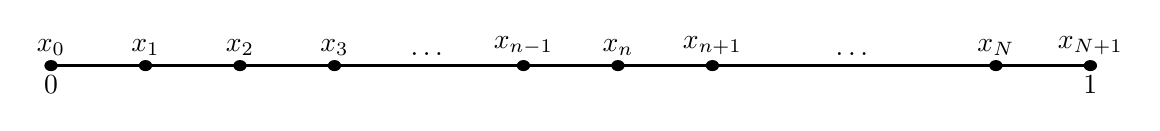
\begin{tikzpicture}[xscale=1.2, yscale=1, thick]
\draw[-] (0,0) -- (11,0);
 \foreach \x in {0,...,3} {
 \fill (\x,0) circle (2pt); % 圆点
 \node[above] at (\x,0) {$x_{\x}$};
 }
 \node[above] at (4,0) {$\dots$};
 \fill (5,0) circle (2pt);
 \node[above] at (5,0) {$x_{n-1}$};
 \fill (6,0) circle (2pt);
 \node[above] at (6,0) {$x_{n}$};
 \fill (7,0) circle (2pt);
 \node[above] at (7,0) {$x_{n+1}$};
 
 \node[above] at (8.5,0) {$\dots$};

 \fill (10,0) circle (2pt);
 \node[above] at (10,0) {$x_{N}$};
 \fill (11,0) circle (2pt);
 \node[above] at (11,0) {$x_{N+1}$};
 
 \node[below] at (0,0) {$0$};
 \node[below] at (11,0) {$1$};
\end{tikzpicture}
\end{center}


The piecewise linear polynomials on such grid is denoted by
\[
X_h^1 := \{v\in C(\bar{I}): v\big |_{I_{n+1}} \in \mathbb{P}_1, \ n=0,\cdots,N \}.
\]
We construct a nodal basis for $X_h^1$, which is based on nodes in every element (how many nodes in every element depends on the degree of freedom, or the degree of polynomials required parameters to be determined). 
\[
\varphi_0 (x) = \left \{
\begin{aligned}
&\frac{x_1-x}{x_1-x_0}, &\quad x\in I_1,\\
& 0, &\quad \text{else},
\end{aligned}
\right.
\qquad 
\varphi_{N+1}(x) = \left\{
\begin{aligned}
& \frac{x-x_N}{x_{N+1}-x_N}, & \quad x\in I_{N+1}, \\
& 0,& \text{else} ,
\end{aligned}
\right .
\]
\[
\varphi_n(x) = \left\{
\begin{aligned}
& \frac{x-x_{n-1}}{x_n-x_{n-1}}, & \quad x\in I_n, \\
& \frac{x_{n+1} - x}{x_{n+1} - x_n}, & \quad x\in I_{n+1}, \\
& 0,&\quad \text{else}.
\end{aligned}
\right.
\]
Clearly, we have $X_h^1 = \mathrm{span}\{\varphi_0,\varphi_1,\cdots,\varphi_{N+1}\}$. For any $u\in C(\bar{I})$, its interpolation into $X_h^1$ is denoted by $u_I(x)$. Clearly, we have $u_I(x) = \sum_{i=0}^{N+1} u(x_i) \varphi_i(x)$ and 
\[
u_I \big |_{I_{n+1}} = u(x_n) \varphi_n(x) + u(x_{n+1}) \varphi_{n+1}(x) =
u(x_n) \frac{x_{n+1}-x}{x_{n+1} - x_n} + u(x_{n+1}) \frac{x-x_n}{x_{n+1}-x_n}.
\]
Let the finite element space $V_h=X_h^1 \cap V$. It is known that $X_h^1\subset H^1(I)$ [see HW 9, Exercise 1], then $V_h=\{v\in X_h^1: v(0)=0\}$, i.e.,
\[
V_h = \mathrm{span}\{\varphi_1,\cdots,\varphi_{N+1}\}.
\]



$\bullet$ FEM Implementation.
Let $u_h = \sum_{j=1}^{N+1} u_j \varphi_j(x)$, then 
\[
\sum_{j=1}^{N+1} u_j a(\varphi_j, \varphi_i) = \mathcal{F}(\varphi_i),\quad i=1,\cdots,N+1.
\]
Let $\mathbf{A} = (a_{i, j})$ be the $(N+1)\times(N+1)$ matrix with its entries $a_{i,j} = a(\varphi_j,\varphi_i)$. Then we have
\[
\begin{aligned}
&a_{N+1,N+1} = \frac{1}{h_{N+1}},\ a_{j,j} = \frac{1}{h_j} + \frac{1}{h_{j+1}}, \quad j=1,\cdots,N, \\
& a_{j,j+1} = a_{j+1,j} = -\frac{1}{h_{j+1}}, \ j=1,\cdots,N, \\
& a_{i,j} = 0,\ \text{if}\ |i-j|\geqslant 2.
\end{aligned}
\]
Thus
\[
\frac{1}{h}
\begin{bmatrix}
2 & -1 & & & \\
-1 & 2 & -1 &&  \\
 & \ddots &\ddots & \ddots & \\
 & & -1 & 2 & -1 \\
 & & & -1 & 1 \\
\end{bmatrix}
\begin{bmatrix}
u_1 \\
u_2 \\
\vdots \\
u_N \\
u_{N+1}
\end{bmatrix}
= 
\begin{bmatrix}
(f,\varphi_1) \\
(f,\varphi_2) \\
\vdots \\
(f,\varphi_N) \\
(f,\varphi_{N+1}) + \beta \\
\end{bmatrix}.
\] 

$\bullet$ Error Estimate. We denote $u_I$ being the interpolation of $u$ into $V_h$, then it is known [see HW 10, Exercise 1] that 
\[
\|u-u_I\|_0 \leqslant Ch \|u^\prime - u_I^\prime\|_0 \leqslant Ch^2 \|u^{\prime\prime}\|_0.
\]
 We know $a(u-u_h, v_h) = 0$ for any $v_h\in V_h$. Then
 \[
 \|u^\prime-u_h^\prime\|_0^2 = a(u-u_h, u-u_h) = a(u-u_h, u-v_h) \leqslant \|u^\prime-u_h^\prime\|_0 \|u^\prime-v_h^\prime\|_0,\quad \forall v_h\in V_h,
 \]
 which leads to
\[
\|u^\prime-u^\prime_h\|_0 \leqslant \inf_{v_h\in V_h} \|u^\prime - v^\prime_h\|_0 \leqslant \|u^\prime - u^\prime_I \|_0 \leqslant Ch \|u^{\prime\prime}\|_0.
\]
In the following, we derive the estimate for $\|u-u_h\|_0$ by using Aubin-Nitsche trick.

 Consider the dual problem: given $r\in L^2(I)$,
 \[
 \left\{
 \begin{aligned}
 &\text{Find}\ \varphi(r)\in V\ \text{such that} \\
 & a(v,\varphi(r)) = (r,v),\quad \forall v\in V.
 \end{aligned}
 \right.
 \]
The dual problem admits a unique solution $\varphi(r)$ since $a(\cdot,\cdot)$ is continuous and coercive.  Moreover, we have
 \[
 a(v,\varphi(r)) = (r,v),\quad \forall v\in C_0^\infty(I),
 \]
if we suppose $\varphi(r)\in H^2(I)$, which gives $(-\varphi^{\prime\prime} (r), v) = (r,v),\ \forall v\in C_0^\infty (I)$, leading to $-\varphi^{\prime\prime}(r) = r$ in $L^2$ since $C_0^\infty(I)$ is dense in $L^2(I)$. \textcolor{gray}{Since for any $v\in L^2(I)$, there exists $\{ v_n\} \subset C_0^\infty(I)$ such that $\lim_{n\to\infty} \|v-v_n\|_0=0$, then $(\varphi^{\prime\prime}(r)+r, v_n) = 0$ and $(\varphi^{\prime\prime}+r,v) \leqslant \|\varphi^{\prime\prime}+r\|_0 \|v-v_n\|_0\to 0$, as $n\to\infty$. Take $v = \varphi^{\prime \prime}(r)+r$ leading to the desired result.} 

Let $\varphi_I(r)$ be the interpolation of $\varphi(r)$ into $V_h$. We have $\| \varphi^{\prime}(r) - \varphi^{\prime}_I(r)\|_0\leqslant Ch \|\varphi^{\prime\prime} (r)\|_0$ and  
\[
\begin{aligned}
\|u-u_h\|_0 & = \sup_{r\in L^2(I), \ r\neq 0} \frac{(r,u-u_h)}{\|r\|_0} = 
\sup_{r\in L^2(I), \ r\neq 0}  \frac{a(u-u_h, \varphi(r))}{\|r\|_0} \\
& = \sup_{r\in L^2(I), \ r\neq 0}  \frac{a(u-u_h, \varphi(r) - \varphi_I (r))}{\|r\|_0} \\
 & \leqslant \sup_{r\in L^2(I), \ r\neq 0}  \frac{\|u^\prime-u^\prime_h\|_0 \|\varphi^\prime(r) - \varphi^\prime_I(r)\|_0 }{\|r\|_0} \\
 & \leqslant C h\|u^\prime-u^\prime_h\|_0 \sup_{r\in L^2(I), \ r\neq 0} \frac{\|\varphi^{\prime\prime}(r)\|_0}{\|r\|_0}  \\
 & \leqslant C h\|u^\prime-u^\prime_h\|_0.
\end{aligned}
\]
\end{proof}





%\newpage
%\section*{Appendix: Notations for Discrete Representation}
% Let $I = [a,b]$. We define the discrete grid points as
%\[
%a=x_0<x_1<\cdots<x_N = b.
%\]
%We introduce the following sets:
%\[
%I_h = \{x_1,\cdots,x_{N-1}\}, \ \bar{I}_h = \{x_0,x_1,\cdots, x_N\}, \ I_h^+ = \{x_1,\cdots,x_N\}.
%\]
%The grid spacing is defined as
%\[
%h_i = x_{i}- x_{i-1}, \quad i=1,\cdots,N.
%\]
%Additionally, we define the averaged grid spacing:
%\[
%\begin{aligned}
%& \bar{h}_i = \frac{1}{2} (h_i+h_{i+1}), \ i=1,\cdots,N-1,\\
%& \bar{h}_0  = \frac{1}{2} h_1, \quad \bar{h}_N = \frac{1}{2} h_N.
%\end{aligned}
%\]
%A discrete function defined on $\bar{I}_h$ is denoted as 
%\[
%v_h = \{v_0,v_1,\cdots, v_N \}.
%\]
%We define the following difference operators:
%\[
%\begin{aligned}
%& (v_i)_{\bar{x}} := v_{i,\bar{x}} : = \frac{v_i-v_{i-1}}{h_i}, \ i =1,\cdots,N, \\
%& (v_i)_x := v_{i, x} := \frac{v_{i+1} - v_i}{h_{i+1}},\ i=0,\cdots,N-1, \\
%&  (v_i)_{\hat{x}} := v_{i, \hat{x}} := \frac{v_{i+1} - v_i}{\bar{h}_{i}},\ i=0,\cdots,N-1.
%\end{aligned}
%\]
%The discrete inner products are given by
%\begin{equation}
%(u_h, v_h)_{I_h} = \sum_{i=1}^{N-1} u_i v_i \bar{h}_i, \
%(u_h, v_h)_{\bar{I}_h} = \sum_{i=0}^{N} u_i v_i \bar{h}_i, \
%(u_h, v_h)_{I^+_h} = \sum_{i=1}^{N} u_i v_i h_i.
%\label{eq:d-ip}
%\end{equation}
%We define the discrete norms as follows:
%\begin{equation}
%\begin{aligned}
%& \|v_h\|_c := \max_{\bar{I}_h} |v_i|,\ \|v_h\|_0 := (v_h,v_h)_{\bar{I}_h}^{1/2}, \\
%& |v_h|_1 := ((v_h)_{\bar{x}}, (v_h)_{\bar{x}})_{I_h^+}^{1/2}, \ \|v_h\|_1^2 = \|v_h\|_0^2 + |v_h|_1^2.
%\end{aligned}
%\label{eq:d-in}
%\end{equation}
%The discrete integral by parts:
%\begin{equation}
%\sum_{i=m+1}^n v_i (w_i)_{\bar{x}} h_i = - \sum_{i=m}^{n-1} (v_i)_x w_i h_{i+1} + v_n w_n - v_m w_m,\ \text{for some} \ 0\leqslant m < n \leqslant N.
%\label{eq:d-ibp}
%\end{equation}
%The discrete Green formula:
%\begin{equation}
%\sum_{i=m+1}^{n-1} \left( (u_i)_{\bar{x}} \right )_{\hat{x}} v_i \bar{h}_i = - \sum_{i=m+1}^n (u_i)_{\bar{x}} (v_i)_{\bar{x}} h_i + (u_n)_{\bar{x}} v_n - (u_m)_x v_m,\ \text{for some} \ 0\leqslant m < n \leqslant N.
%\label{eq:d-gf}
%\end{equation}
%The discrete Cauchy-Schwarz inequality states that
%\begin{equation}
%|(u_h, v_h)_{\bar{I}_h}| \leqslant (u_h, u_h)_{\bar{I}_h}^{1/2} (v_h, v_h)_{\bar{I}_h}^{1/2}.
%\label{eq:d-csi}
%\end{equation}
%If $v_0 = 0$ (or $v_N=0$ or $v_0=v_N=0$), the discrete Poincar\'e inequality holds:
%\begin{equation}
%\|v_h\|_c \leqslant C |v_h|_1, \quad \|v_h\|_0 \leqslant C |v_h|_1,
%\label{eq:d-pi}
%\end{equation}
%where $C$ is a constant depending only on $a$ and $b$.
%

\end{document}

